\documentclass[11pt,letterpaper]{article}
\usepackage[margin=2cm]{geometry}
\usepackage{amsmath,amssymb,graphicx,xcolor,booktabs,tabularx,enumitem,titlesec,fancyhdr,array,longtable}
\usepackage{caption}
\usepackage{tikz}
\usetikzlibrary{arrows.meta,positioning,shapes.geometric,calc,decorations.pathmorphing,patterns}
\usepackage[hidelinks]{hyperref}
\usepackage{helvet}\renewcommand{\familydefault}{\sfdefault}
\usepackage{microtype}
\titleformat{\section}{\Large\bfseries\color{blue!50!black}}{\thesection}{0.6em}{}
\titleformat{\subsection}{\large\bfseries}{\thesubsection}{0.6em}{}
\titleformat{\subsubsection}{\normalsize\bfseries}{\thesubsubsection}{0.6em}{}
\setlength{\headheight}{14pt}
\pagestyle{fancy}\fancyhf{}\lhead{sPHENIX Self-Paced Course}\rhead{Module 3: Calorimeters}\cfoot{\thepage}
\newcommand{\conceptbox}[2]{\par\medskip\noindent\fcolorbox{blue!50!black}{blue!5}{\begin{minipage}{0.96\linewidth}\textbf{#1}\par\smallskip #2\end{minipage}}\par\medskip}
\newcommand{\connectbox}[1]{\par\medskip\noindent\fcolorbox{green!40!black}{green!5}{\begin{minipage}{0.96\linewidth}\textbf{Connect to your analysis}\par\smallskip #1\end{minipage}}\par\medskip}
\newcommand{\pitfallbox}[1]{\par\medskip\noindent\fcolorbox{red!50!black}{red!4}{\begin{minipage}{0.96\linewidth}\textbf{Pitfalls}\par\smallskip #1\end{minipage}}\par\medskip}
\newcommand{\checksbox}[1]{\par\medskip\noindent\fcolorbox{orange!60!black}{orange!5}{\begin{minipage}{0.96\linewidth}\textbf{Checks}\par\smallskip #1\end{minipage}}\par\medskip}
\newcommand{\workedbox}[2]{\par\medskip\noindent\fcolorbox{gray!60!black}{gray!6}{\begin{minipage}{0.96\linewidth}\textbf{Worked example: #1}\par\smallskip #2\end{minipage}}\par\medskip}
\newcommand{\goal}[1]{\par\noindent\textbf{Goal.} #1\par\smallskip}
\newcommand{\code}[1]{\texttt{#1}}
\setlist{itemsep=1pt,topsep=3pt}
\setlength{\emergencystretch}{3em}
\setlength{\parskip}{3pt}
\captionsetup{font=small}
\begin{document}
\begin{center}{\LARGE\bfseries sPHENIX Self-Paced Course --- Module 3}\\[4pt]
{\Large Calorimetry in sPHENIX: EMCal and HCal hardware}\\[8pt]
Prepared for P.\,D.\ Lewis (Ohio University) \quad November 2026\\[2pt]
\small Self-contained study text built on the Summer-2026 sPHENIX School, public sPHENIX papers and standard calorimetry textbooks\end{center}

\tableofcontents
\newpage

\section*{How to use this module}
\addcontentsline{toc}{section}{How to use this module}
This module is self-contained.
Everything you need is explained in the text, from first principles to the way sPHENIX actually does it.
You do not need to open slides, recordings or papers to follow it.
The school talks listed below are the \emph{sources} the module was built from; they are cited as [S\#\#] so that you can trace a statement if you ever want to.

\subsection*{Learning objectives}
After this module you should be able to:
\begin{enumerate}[label=O\arabic*.]
\item Explain how electromagnetic and hadronic showers develop, using the radiation length $X_0$, the Moli\`ere radius $R_M$, the critical energy $E_c$ and the nuclear interaction length $\lambda_I$.
\item Explain what a sampling calorimeter is, define the sampling fraction, and estimate the stochastic term from the sampling geometry.
\item Describe the sPHENIX EMCal (tungsten-powder/scintillating-fibre SPACAL blocks, 2D projectivity, light guides, SiPMs) and its tower grid of $96\times256$ in $\eta\times\phi$.
\item Describe the inner and outer HCal (aluminium frame and steel flux return, tilted plates, scintillating tiles with wavelength-shifting fibres, $24\times64$ towers per layer).
\item Follow the signal chain from photon in the fibre to a calibrated \code{TowerInfo} object: SiPM, preamplifier, digitiser, waveform, template fit, status, calibration.
\item Decompose the energy resolution into stochastic, constant and noise terms, and say which hardware or calibration effect feeds each term.
\item Outline the calibration chain: test beam, LED and cosmic tests, cosmic-muon MIP scale for the HCal, tower-slope relative calibration, $\pi^0$ calibration for the EMCal, temperature and timing corrections.
\item Connect all of the above to the $\pi^0$ and $\eta$ peaks you measure in your own analysis.
\end{enumerate}

\subsection*{Prerequisites and time}
Modules 1 (physics programme) and 2 (RHIC and detector overview).
Estimated time: 9--11 hours (about 6 hours of reading, 2 hours for the worked examples, 1--3 hours for the optional exercises).

\subsection*{Sources (sPHENIX School 2026, BNL, July 2026)}
\begin{itemize}
\item {[S09]} C. Woody, ``EMCal Overview'' --- the main EMCal hardware source.
\item {[S08]} J. Haggerty, ``HCal and Global Detector Overview'' --- HCal design, tiles, test beams, LEDs, lessons learned.
\item {[S47]} B. Seidlitz, J. Nagle, S. Bathe, ``Calorimeter test-beam simulation'' (workfest) --- how to read test-beam results.
\item {[S42]} A. M. Khan, ``HCal Calibration studies'' (flash talk) --- the tower-slope method.
\item Also used for the calibration overview: [S15] B. Seidlitz, ``EMCal Reco and Calibrations''; [S16] A. Menon, ``HCal Reco and Calibrations''. Module 7 treats reconstruction in depth.
\end{itemize}

\subsection*{Public readings (optional)}
Aidala et al., IEEE TNS 65 (2018) 2901, arXiv:1704.01461 (prototype design and beam tests) [R1];
Aidala et al., IEEE TNS 68 (2021) 173, arXiv:2003.13685 (2D-projective EMCal prototype) [R2];
the sPHENIX proposal, arXiv:1501.06197 [R3]; the PDG review of particle detectors and passage of particles through matter [R4].

\conceptbox{Notation used throughout}{Energies in GeV unless stated. $\oplus$ means addition in quadrature: $a\oplus b=\sqrt{a^2+b^2}$.
``Tower'' means the smallest read-out cell of a calorimeter. ``Block'' (EMCal) means one machined tungsten/fibre piece containing $2\times2$ towers.
$\eta$ is pseudorapidity, $\phi$ azimuth; ``$i\eta$, $i\phi$'' are integer tower indices.}

%=====================================================================
\section{Why calorimetry, and what sPHENIX needed}\label{sec:req}
\goal{Understand which physics measurements set the calorimeter requirements, and why they lead to a compact, projective, finely segmented EMCal and a two-layer HCal built into the magnet return yoke.}

\subsection{What a calorimeter does}
A calorimeter measures the energy of a particle by stopping it completely.
The particle interacts with dense material and produces a cascade (a ``shower'') of lower-energy secondaries.
Eventually all of the energy is converted into ionisation and excitation of atoms, plus some invisible losses.
A fraction of that deposited energy is turned into a measurable signal, here scintillation light.
The signal is proportional to the incident energy, so one number (the calibration constant) converts signal to energy.

Calorimeters have three properties that trackers do not have.
First, they measure neutral particles (photons, neutrons, $K^0_L$).
Second, their relative resolution \emph{improves} with energy, as $1/\sqrt{E}$, while a tracker's momentum resolution degrades as $p$ grows.
Third, they are fast and can be used to trigger: a large energy deposit is a simple signature for a high-$p_T$ photon or jet (Module 5).

There are two kinds of showers, electromagnetic (photons, electrons) and hadronic (pions, protons, neutrons, \dots).
There are two kinds of calorimeters: \emph{homogeneous} (the whole volume is active, e.g.\ a lead-glass or crystal block) and \emph{sampling} (layers or fibres of active material embedded in a passive, dense absorber).
Both sPHENIX calorimeters are sampling calorimeters [S09, S08].

\subsection{Physics drivers}
The sPHENIX calorimeter system was designed around three classes of measurements [S09, S08, R3]:
\begin{enumerate}
\item \textbf{Jets} in $p$+$p$, $p$+Au and Au+Au. Jets need both the electromagnetic part (mostly photons from $\pi^0$ decays) and the hadronic part of the energy. This drives full azimuthal coverage, $|\eta|<1.1$, and a hadronic calorimeter.
\item \textbf{Direct photons and $\pi^0$} (your physics). These need an EMCal with good energy resolution, a small shower size and fine segmentation.
\item \textbf{$\Upsilon\to e^+e^-$}. Electrons of about 5 GeV must be identified against a large hadron background, using $E/p$ (EMCal energy over track momentum) and shower shape.
\end{enumerate}
The energy range is modest compared with the LHC: roughly 1 to 100 GeV for single particles and roughly 20 to 70 GeV for jets [S08].
The design goals were an EMCal resolution of about $15\%/\sqrt{E}$ and a single-hadron HCal resolution of order $100\%/\sqrt{E}$ [S09, R3].

\subsection{The underlying event sets the scale}
In central Au+Au collisions thousands of soft particles are produced.
Every tower receives some energy from this ``underlying event'' (UE), and that energy fluctuates.
For a photon or electron cluster, what matters is the UE energy inside the cluster area and its fluctuation.
The smaller the cluster area, the smaller this background.
Hence the EMCal must have a small Moli\`ere radius and small towers.

\workedbox{UE energy under a cluster (toy)}{Take a transverse-energy density at midrapidity of order $\mathrm{d}E_T/\mathrm{d}\eta\approx 600$ GeV in the most central Au+Au events (the order of magnitude measured at RHIC; see the public sPHENIX $E_T$ paper [R5] for the actual values).
Spread uniformly in $\phi$, this is $600/(2\pi)\approx 95$ GeV per unit of $\eta$ per radian.
A $3\times3$ EMCal tower array covers $\Delta\eta\times\Delta\phi=0.075\times0.074\approx 0.0055$.
The UE then deposits roughly $95\times0.0055\approx 0.5$ GeV in the cluster area (only part of it in the EMCal, since hadrons pass through).
Compare: a 5 GeV electron measured with $15\%/\sqrt{E}$ has $\sigma_E\approx0.15\sqrt{5}\approx0.34$ GeV.
\emph{Conclusion:} the UE contribution is comparable to the detector resolution. Making the cluster area four times larger would make the UE dominate. This is why the EMCal is compact and finely segmented. (Toy numbers; illustrative only.)}

\subsection{Mechanical constraints}
sPHENIX re-uses the former BaBar superconducting solenoid (1.4 T) [S09, R3].
Early designs put the solenoid inside the calorimeters; the final design places the EMCal and the inner HCal \emph{inside} the solenoid and the outer HCal outside it [S09].
Three consequences follow:
\begin{itemize}
\item The EMCal sits close behind the tracker, with little material in front. Photons have less chance to convert or shower before the EMCal.
\item The EMCal inner radius is about 90 cm, set by the need for space for the tracker and by occupancy in Au+Au; the outer radius is about 116 cm. The EMCal therefore has only about 26 cm of radial space, including electronics, so it must be very dense [S09].
\item The outer HCal steel doubles as the magnet's flux return. This is economical: the return yoke is needed anyway, so instrumenting it gives a hadronic calorimeter at low cost [S08, S09].
\end{itemize}

\subsection{Projectivity}
A tower is \emph{projective} if its long axis points back to the interaction point.
A particle from the vertex then travels along the tower axis, and its shower stays in few towers.
In a non-projective geometry, a particle at large $|\eta|$ enters at an angle; its shower crosses several towers in depth and looks wider.
sPHENIX chose an approximately \emph{two-dimensional} projective EMCal: towers are tilted in both $\eta$ and $\phi$ [S09].
At $\eta\approx 0$, a one-dimensional projective design would be almost as good.
At $|\eta|\to1$ the 2D projectivity keeps the transverse shower size small, which improves energy resolution and electron--hadron separation in the high-multiplicity environment [S09, R2].

\begin{figure}[h]\centering
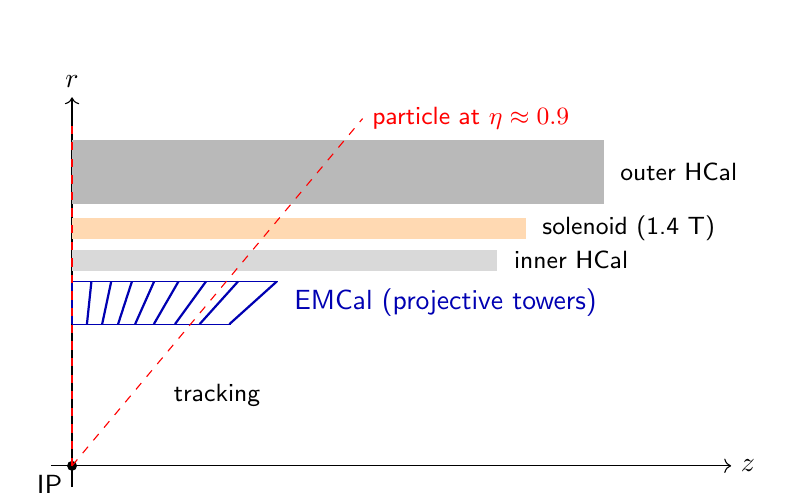
\begin{tikzpicture}[scale=0.9]
\draw[->] (-0.3,0) -- (9.3,0) node[right] {$z$};
\draw[->] (0,-0.3) -- (0,5.2) node[above] {$r$};
\fill (0,0) circle (2pt) node[below left] {IP};
% EMCal projective towers
\foreach \th in {90,84,78,72,66,60,54,48,42}{
  \pgfmathsetmacro{\c}{cos(\th)}\pgfmathsetmacro{\s}{sin(\th)}
  \pgfmathsetmacro{\ra}{2.0/\s}\pgfmathsetmacro{\rb}{2.6/\s}
  \draw[blue!70!black,thick] ({\ra*\c},2.0) -- ({\rb*\c},2.6);
}
\draw[blue!70!black] (0,2.0) -- (2.25,2.0); \draw[blue!70!black] (0,2.6) -- (2.9,2.6);
\node[blue!70!black,anchor=west] at (3.0,2.3) {EMCal (projective towers)};
\fill[gray!30] (0,2.75) rectangle (6.0,3.05); \node[anchor=west] at (6.1,2.9) {\small inner HCal};
\fill[orange!30] (0,3.2) rectangle (6.4,3.5); \node[anchor=west] at (6.5,3.35) {\small solenoid (1.4 T)};
\fill[gray!55] (0,3.7) rectangle (7.5,4.6); \node[anchor=west] at (7.6,4.15) {\small outer HCal};
\draw[dashed,red] (0,0) -- (4.1,4.9) node[right,red] {\small particle at $\eta\approx0.9$};
\draw[dashed,red] (0,0) -- (0,4.8);
\node[anchor=west] at (1.3,1.0) {\small tracking};
\end{tikzpicture}
\caption{Schematic $r$--$z$ quarter view (not to scale). EMCal towers point back towards the interaction point (IP). The inner HCal and the EMCal are inside the solenoid; the outer HCal is outside and acts as the flux return.}\label{fig:rz}
\end{figure}

\checksbox{You should be able to answer: Why is the EMCal inside the magnet? (Less material in front; compact.) Why must it be dense? (Little radial space, small showers for UE.) Why does the HCal live in the return yoke? (Cost and space.)}

%=====================================================================
\section{Electromagnetic showers}\label{sec:em}
\goal{Be able to estimate, with pencil and paper, where a photon shower starts, where it peaks, how deep and how wide it is, and how much of it a block of given size contains.}

\subsection{Interactions of electrons and photons}
Above a few tens of MeV, electrons and positrons lose energy mainly by \emph{bremsstrahlung}: they radiate photons in the Coulomb field of nuclei.
Photons above a few MeV interact mainly by \emph{pair production}, $\gamma\to e^+e^-$, again in the nuclear field.
Both processes are governed by the same material constant, the \textbf{radiation length} $X_0$.
\begin{itemize}
\item An electron loses on average a fraction $1-1/e$ of its energy by bremsstrahlung in one $X_0$: $\langle E(x)\rangle=E_0\,e^{-x/X_0}$.
\item A high-energy photon has a mean free path for pair production of $\tfrac{9}{7}X_0$.
\end{itemize}
A useful approximation for $X_0$ is [R4]
\begin{equation}
X_0\approx\frac{716.4\ \mathrm{g\,cm^{-2}}\;A}{Z(Z+1)\ln(287/\sqrt{Z})}.
\end{equation}
It falls roughly as $1/Z^2$, so high-$Z$ materials such as tungsten ($Z=74$) or lead ($Z=82$) are compact.
For tungsten this gives about 6.8 g/cm$^2$, i.e.\ 0.35 cm at a density of 19.3 g/cm$^3$.

Below the \textbf{critical energy} $E_c$, ionisation losses exceed radiation losses, and the electrons simply range out.
Roughly $E_c\approx 610\ \mathrm{MeV}/(Z+1.24)$ for solids; for tungsten $E_c\approx 8$ MeV [R4].

\subsection{The Heitler toy model}
A simple model captures the essentials.
Assume that after every $X_0$ each particle splits into two of half the energy (an electron radiates one photon; a photon converts into a pair).
After $t$ radiation lengths there are $N(t)=2^t$ particles of energy $E_0/2^t$.
Multiplication stops when the energy per particle reaches $E_c$.
This gives
\begin{equation}
t_{\max}=\frac{\ln(E_0/E_c)}{\ln2},\qquad N_{\max}=\frac{E_0}{E_c}.
\end{equation}
Two lessons follow.
The depth of the shower maximum grows only \emph{logarithmically} with energy, so a calorimeter of fixed depth contains showers over a wide energy range.
The number of charged particles, and hence the signal, is \emph{proportional} to $E_0$, which is the basis of calorimetry.
The total track length of charged particles is $\propto E_0/E_c\cdot X_0$; fluctuations in this number set the ultimate (intrinsic) resolution.

\subsection{Longitudinal profile}
A better description, fitted to simulations, is a gamma distribution [R4]:
\begin{equation}
\frac{1}{E_0}\frac{\mathrm{d}E}{\mathrm{d}t}=\frac{b\,(bt)^{a-1}e^{-bt}}{\Gamma(a)},\qquad t=x/X_0,\qquad t_{\max}=\frac{a-1}{b},
\end{equation}
with $b\approx0.5$ and
\begin{equation}
t_{\max}\approx\ln\frac{E_0}{E_c}+C_j,\qquad C_e=-0.5,\quad C_\gamma=+0.5 .
\end{equation}
Photons shower about one $X_0$ later than electrons, because the photon must first convert.
The fraction of energy contained in a depth $T$ is the regularised incomplete gamma function $P(a,bT)$.

\begin{figure}[h]\centering
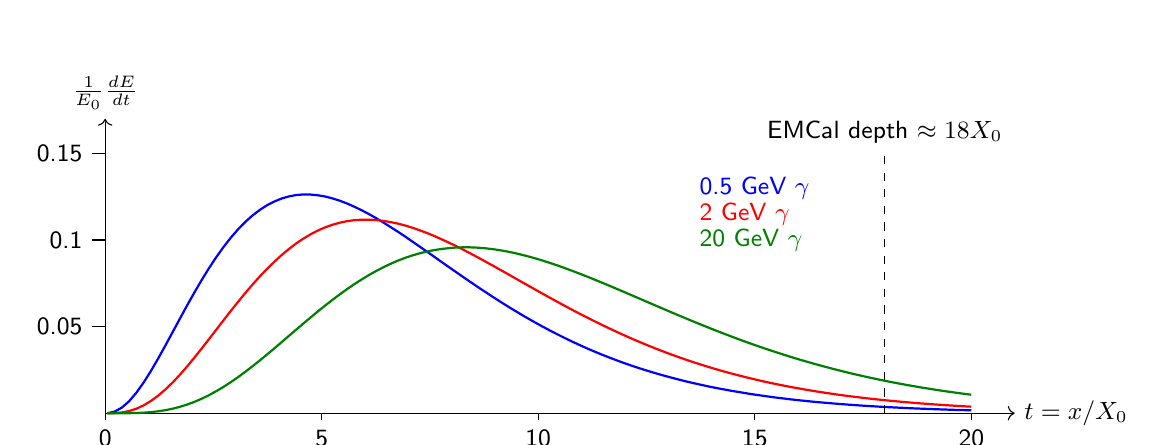
\begin{tikzpicture}[xscale=0.55,yscale=22]
\draw[->] (0,0) -- (21,0) node[right] {\small $t=x/X_0$};
\draw[->] (0,0) -- (0,0.17) node[above] {\small $\frac{1}{E_0}\frac{dE}{dt}$};
\foreach \x in {0,5,10,15,20} \draw (\x,0) -- (\x,-0.004) node[below] {\small \x};
\foreach \y in {0.05,0.1,0.15} \draw (0,\y) -- (-0.3,\y) node[left] {\small \y};
% a=3.32 (0.5 GeV), a=4.01 (2 GeV), a=5.16 (20 GeV); b=0.5
\draw[thick,blue,domain=0.05:20,samples=120] plot (\x,{0.5*exp(2.32*ln(0.5*\x)-0.5*\x)/2.740});
\draw[thick,red,domain=0.05:20,samples=120] plot (\x,{0.5*exp(3.01*ln(0.5*\x)-0.5*\x)/6.076});
\draw[thick,green!50!black,domain=0.05:20,samples=120] plot (\x,{0.5*exp(4.16*ln(0.5*\x)-0.5*\x)/30.63});
\draw[dashed] (18,0) -- (18,0.15) node[above] {\small EMCal depth $\approx18X_0$};
\node[blue,anchor=west] at (13.5,0.13) {\small 0.5 GeV $\gamma$};
\node[red,anchor=west] at (13.5,0.115) {\small 2 GeV $\gamma$};
\node[green!50!black,anchor=west] at (13.5,0.10) {\small 20 GeV $\gamma$};
\end{tikzpicture}
\caption{Toy longitudinal profiles from the gamma-function parametrisation with $b=0.5$ and $E_c=8$ MeV (pure-tungsten value). Schematic; not sPHENIX data.}\label{fig:long}
\end{figure}

\subsection{Lateral profile and the Moli\`ere radius}
The shower spreads sideways mainly through multiple Coulomb scattering of the low-energy electrons.
The natural transverse scale is the \textbf{Moli\`ere radius}
\begin{equation}
R_M\approx X_0\,\frac{21.2\ \mathrm{MeV}}{E_c}.
\end{equation}
About 90\% of the energy lies inside a cylinder of radius $1\,R_M$ around the shower axis, and about 95\% inside $2\,R_M$ [R4].
The lateral profile has a narrow core (from the early, energetic part of the shower) and a broad halo (from low-energy photons travelling far before converting).
$R_M$ is nearly independent of the incident energy, and it depends on $X_0/E_c\propto A/Z$ rather than on $Z^2$, so it is less sensitive to the material than $X_0$.

\subsection{Numbers for the sPHENIX EMCal}
The sPHENIX EMCal absorber is a mixture of tungsten powder and epoxy with embedded scintillating fibres.
Its density is about 9--10 g/cm$^3$, giving $X_0\approx7$ mm and $R_M\approx2.3$ cm, with a total depth of about 18 $X_0$ [S09, R1].
The mixture has a lower average $Z$ than pure tungsten, so its $E_c$ is somewhat higher than 8 MeV and showers peak slightly earlier than the pure-tungsten estimate below. The estimate is therefore conservative.

\workedbox{containment of a 2 GeV photon (checkpoint exercise)}{\textbf{Longitudinal.} $t_{\max}=\ln(2000/8)+0.5=5.5+0.5=6.0\,X_0$, i.e.\ about 4.2 cm into the block. With $b=0.5$, $a=1+b\,t_{\max}=4.0$.
The fraction inside $T=18\,X_0$ is $P(4.0,\,9)=1-e^{-9}(1+9+9^2/2+9^3/6)\approx 0.98$.
So about 2\% leaks out of the back. For 20 GeV ($a\approx5.2$) the leakage grows to about 6\%; for 0.5 GeV it is about 1\%.\\[3pt]
\textbf{Lateral.} The tower front face is about $\Delta\phi\times R=2\pi/256\times93\ \mathrm{cm}\approx2.3$ cm, i.e.\ about $1\,R_M$.
A $3\times3$ array centred on the shower extends $\pm1.5$ towers $\approx\pm1.5\,R_M$ from the axis. Interpolating between the 90\% ($1R_M$) and 95\% ($2R_M$) rules gives about 92--93\% containment (somewhat less if the photon hits a tower corner, since the $3\times3$ is then off-centre).\\[3pt]
\textbf{Total.} Roughly $0.98\times0.93\approx0.91$ of the energy is inside a $3\times3$ array. A $5\times5$ array ($\pm2.5R_M$) recovers about 96--97\% laterally.\\[3pt]
\textbf{Lesson.} The ``raw'' cluster energy is several percent below the true energy, and the missing fraction depends on energy and impact position. The energy calibration (Section~\ref{sec:calib}) and the simulation must account for it consistently. (Approximate textbook model; not a sPHENIX measurement.)}

\subsection{Two photons from a $\pi^0$}
For a $\pi^0$ of energy $E$, the minimum opening angle of the two decay photons is $\theta_{\min}\approx 2m_{\pi^0}/E$.
At $E=5$ GeV this is $0.054$ rad, i.e.\ about 5 cm at $R=93$ cm, or about two tower widths.
At $E=10$ GeV it is about one tower width.
At higher energy the two showers merge into one cluster.
The small $R_M$ and the small towers of the sPHENIX EMCal push this merging threshold up; above it, $\pi^0$ identification relies on shower shape rather than on two separate clusters.

\connectbox{Your $\pi^0$/$\eta\to\gamma\gamma$ reconstruction uses the invariant mass
$m^2=2E_1E_2(1-\cos\theta_{12})$.
Lateral leakage outside the cluster lowers $E_1$ and $E_2$, and so shifts the reconstructed peak below $m_{\pi^0}$ unless the calibration absorbs it.
Because the merging of the two photons sets in at high $p_T$, your $\pi^0$ efficiency from PYTHIA8 with EMCal smearing must reproduce the cluster splitting/merging; this is one reason the simulation must model the shower width correctly. The $\eta$ meson ($m_\eta\approx548$ MeV, four times heavier) opens up four times more, so it merges at much higher energy.}

\pitfallbox{\begin{itemize}
\item Using the pure-tungsten $X_0$ (3.5 mm) for the EMCal: the powder/epoxy/fibre mixture has $X_0\approx7$ mm.
\item Forgetting that photons shower about one $X_0$ later than electrons.
\item Treating lateral containment as energy-independent: the core is nearly energy-independent, but the leakage of the halo and of the back of the shower is not.
\end{itemize}}

%=====================================================================
\section{Sampling calorimetry and energy resolution}\label{sec:samp}
\goal{Know what sets the energy resolution of a sampling calorimeter, be able to estimate each term, and know which term each hardware or calibration choice affects.}

\subsection{Sampling fraction}
In a sampling calorimeter only the active medium produces a signal.
The \textbf{sampling fraction} is
\begin{equation}
f_{\rm samp}=\frac{E_{\rm dep}(\text{active})}{E_{\rm dep}(\text{active})+E_{\rm dep}(\text{absorber})}.
\end{equation}
For a minimum-ionising particle (MIP) it can be computed from the $\mathrm{d}E/\mathrm{d}x$ and thicknesses of the two media.
For electromagnetic showers the actual value is usually somewhat smaller than the MIP value, because the many soft photons in a shower are absorbed preferentially in the high-$Z$ absorber (photoelectric effect scales as $Z^{4-5}$).
The sPHENIX EMCal has $f_{\rm samp}\approx2\%$: only about one fiftieth of the shower energy is deposited in the fibres [S09, R1].
The HCal sampling fraction is a few percent and, because the scintillating tiles are flat while the steel plates are tapered, it changes with depth [S08].

\subsection{The resolution formula}
The relative energy resolution of a calorimeter is written as
\begin{equation}
\frac{\sigma_E}{E}=\frac{a}{\sqrt{E}}\oplus b\oplus\frac{c}{E}.\label{eq:res}
\end{equation}
\begin{itemize}
\item \textbf{Stochastic term $a$.} Any Poisson-like fluctuation in the number of independent signal quanta $N\propto E$ gives $\sigma_N/N=1/\sqrt{N}\propto1/\sqrt{E}$. In a sampling calorimeter the dominant sources are \emph{sampling fluctuations} (how many shower particles happen to cross the active medium) and \emph{photostatistics} (how many photoelectrons are produced).
\item \textbf{Constant term $b$.} Effects proportional to $E$: tower-to-tower calibration errors, non-uniform response across the tower face or along the depth, leakage that fluctuates proportionally. This term dominates at high energy.
\item \textbf{Noise term $c$.} An energy-independent noise $\sigma_{\rm noise}$ (electronics, pedestal width, pile-up, underlying event) gives $\sigma_E/E=\sigma_{\rm noise}/E$. It dominates at low energy.
\end{itemize}
The terms add in quadrature because they are independent.

\subsection{Estimating the sampling term}
A widely used empirical rule for electromagnetic sampling calorimeters [R6] is
\begin{equation}
\frac{a_{\rm samp}}{\sqrt{E}}\approx 2.7\%\sqrt{\frac{d\,[\mathrm{mm}]}{f_{\rm samp}}}\;\frac{1}{\sqrt{E\,[\mathrm{GeV}]}},
\end{equation}
where $d$ is the thickness of the active layers (here, the fibre diameter).
The reasoning: the number of independent crossings of the active medium is proportional to $E\,f_{\rm samp}/d$; finer sampling (smaller $d$) at the same $f_{\rm samp}$ gives more crossings and smaller fluctuations.

\workedbox{sampling term of the sPHENIX EMCal}{Fibres of 0.47 mm diameter and $f_{\rm samp}\approx0.02$ give $a_{\rm samp}\approx2.7\%\sqrt{0.47/0.02}=2.7\%\times4.85\approx13\%$.
Add photostatistics: if a tower produces $N_{\rm pe}$ photoelectrons per GeV, the contribution is $1/\sqrt{N_{\rm pe}}$. For a toy value of 400 p.e./GeV this is 5\%. Then $a\approx13\%\oplus5\%\approx14\%$.
This is close to the 15\% design goal, which shows that the fibre geometry, not the photodetector, sets the stochastic term. (Rule-of-thumb estimate.)}

\subsection{Measured resolutions in beam tests}
The prototypes were measured at the Fermilab Test Beam Facility (experiment T-1044) between 2014 and 2018 [S09, S08, R1, R2].
Public results:
\begin{itemize}
\item 2016 prototype at $\eta\approx0$, electrons in the EMCal: $\sigma_E/E=2.8\%\oplus15.5\%/\sqrt{E}$ [R1].
\item Same campaign, hadrons in the combined EMCal+HCal: $\sigma_E/E=13.5\%\oplus64.9\%/\sqrt{E}$ [R1].
\item 2018 2D-projective EMCal prototype at $\eta\approx1$: $3.5\%\oplus13.3\%/\sqrt{E}$ or $3.0\%\oplus15.4\%/\sqrt{E}$, depending on the position-dependent correction used [R2].
\end{itemize}

\workedbox{what $2.8\%\oplus15.5\%/\sqrt{E}$ means for your photons}{
\begin{tabular}{@{}lcccccc@{}}\toprule
$E$ (GeV) & 1 & 2 & 5 & 10 & 20 & 30\\\midrule
$\sigma_E/E$ (\%) & 15.8 & 11.3 & 7.5 & 5.6 & 4.5 & 4.0\\
$\sigma_E$ (GeV) & 0.16 & 0.23 & 0.37 & 0.56 & 0.89 & 1.19\\\bottomrule
\end{tabular}\\[4pt]
At 2 GeV the stochastic term is $15.5/\sqrt2=11.0\%$ and dominates; at 30 GeV it is $2.8\%$, equal to the constant term. For most $\pi^0$ photons in $p$+$p$ (a few GeV) the stochastic term matters most; at the highest $p_T$ the constant term, i.e.\ calibration quality, takes over.}

\subsection{From photon resolution to $\pi^0$ mass resolution}
Differentiate $m^2=2E_1E_2(1-\cos\theta)$:
\begin{equation}
\frac{\sigma_m}{m}=\frac12\left[\frac{\sigma_{E_1}}{E_1}\oplus\frac{\sigma_{E_2}}{E_2}\oplus\frac{\sigma_\theta}{\tan(\theta/2)}\right].
\end{equation}
For a symmetric decay with $E_1=E_2=2$ GeV, the energy part alone gives $\tfrac12\sqrt2\times11.3\%\approx8\%$ of $m_{\pi^0}$, about 11 MeV.
The angular term adds to this; it comes from the cluster position resolution, which in turn depends on tower size and shower shape.
In real data the peak is also broadened by the underlying event (Au+Au), by miscalibration (constant term), and by non-linearity.

\connectbox{The width of your $\pi^0$ peak is a direct read-out of the photon resolution.
In your PYTHIA8 efficiency, the ``EMCal smearing'' is the extra Gaussian smearing added to simulated cluster energies (and positions) until the simulated $\pi^0$ and $\eta$ widths match data [S15].
If the smearing is too small, the simulated efficiency for a given mass window is too high. If your analysis uses a fixed mass window, a mismatch in width between data and MC is a direct systematic on the cross section.}

\subsection{Linearity}
A calorimeter is linear if the mean signal is proportional to the incident energy.
Sources of non-linearity in sPHENIX are (i) SiPM saturation, since each SiPM has a finite number of pixels (Section~\ref{sec:sipm}); (ii) the readout electronics range; (iii) energy-dependent leakage [S09].
The EMCal prototypes showed a measurable non-linearity at high energy, attributed to SiPM saturation and electronics [S09, R2].
The non-linearity affects exactly the high-energy region where single photons are measured, so it must be modelled.

\pitfallbox{\begin{itemize}
\item Reading a test-beam ``resolution vs energy'' plot without checking how each point was normalised. If each energy point was rescaled so that its mean equals the beam energy, the plot only tests the \emph{shape} (width) of the response, and tells you nothing about linearity or the absolute data-to-MC scale [S47]. Linearity must be shown with a single energy-independent scale factor.
\item Comparing resolutions with different beam spot sizes: a small beam spot centred on a tower gives a better resolution than a beam spread over the tower face, because of the position dependence of the response [S09, R2].
\item Forgetting that $\oplus$ is quadrature: $2.8\%\oplus15.5\%/\sqrt{E}$ is \emph{not} $2.8\%+15.5\%/\sqrt{E}$.
\end{itemize}}

%=====================================================================
\section{The sPHENIX EMCal}\label{sec:emcal}
\goal{Know how the EMCal is built, from fibre to sector, and why each choice was made.}

\subsection{The SPACAL concept}
A \emph{spaghetti calorimeter} (SPACAL) is a sampling calorimeter in which the active medium is a dense array of scintillating fibres running (nearly) along the particle direction, embedded in an absorber [S09].
The idea was developed in the 1980s (e.g.\ by the SPACAL collaboration, with lead absorber) and used in several experiments.
Earlier SPACALs grooved lead plates and laid fibres into them.
sPHENIX introduced a new variant: a matrix of \textbf{tungsten powder and epoxy}, cast around the fibres [S09].
This is denser than lead SPACAL, so the calorimeter fits into the available 26 cm of radius.
The sPHENIX EMCal was the first W/SciFi SPACAL deployed in a running experiment [S09].

\subsection{Blocks, towers and sectors}
\begin{itemize}
\item \textbf{Fibres:} 0.47 mm diameter, about 1 mm apart, from two vendors [S09].
\item \textbf{Block fabrication:} a mould holds the fibre array (positioned by metal meshes along its length); tungsten powder is poured in and the mould is infused with epoxy; the block is then machined to its final tapered shape [S09].
\item \textbf{Block = $2\times2$ towers.} Each block is read out as four towers [S09, R2].
\item \textbf{Totals:} 6144 blocks $\times$ 4 = 24\,576 towers, arranged as 96 towers in $\eta$ times 256 towers in $\phi$, covering $|\eta|<1.1$ and $2\pi$ [S09].
\item \textbf{Tower size:} $\Delta\eta\times\Delta\phi\approx0.025\times0.025$ ($2\pi/256=0.0245$ rad).
\item \textbf{Sectors:} 64 sectors, two in $\eta$ (north/south half) times 32 in $\phi$ [S09]. Each sector covers $8$ towers in $\phi$ ($256/32$) and $48$ in $\eta$ ($96/2$).
\item \textbf{Production:} the mid-rapidity blocks ($|\eta|<0.85$) were produced at UIUC, and the high-rapidity blocks ($0.85<|\eta|<1.1$) in China. Modules and sectors were assembled and tested at BNL; installation ran from 2022 [S09].
\end{itemize}

\begin{figure}[h]\centering
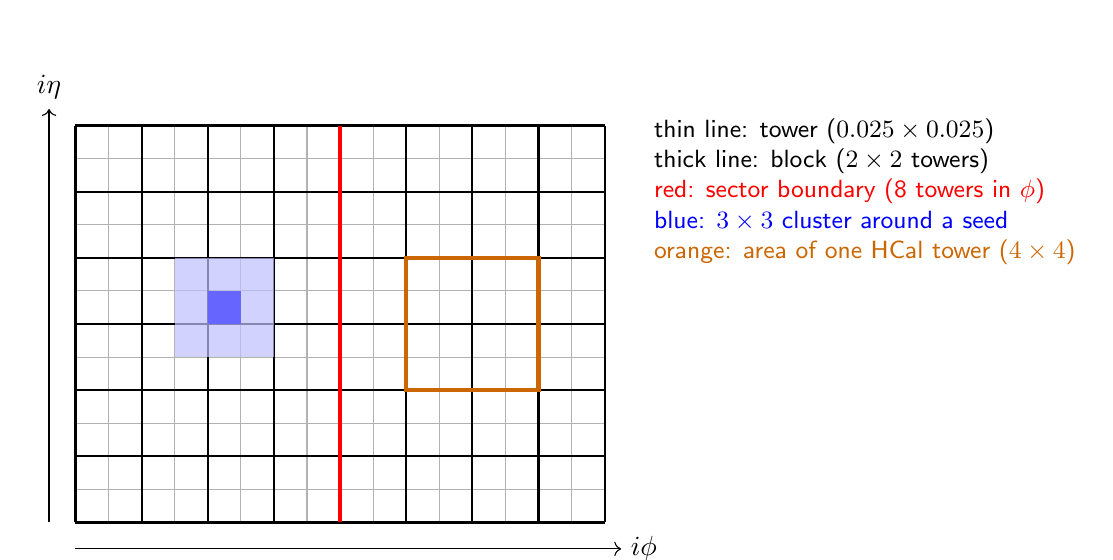
\begin{tikzpicture}[scale=0.42]
% tower grid schematic: draw a patch of 16x12 towers with block boundaries and a sector boundary
\foreach \i in {0,...,16} \draw[gray!60] (\i,0) -- (\i,12);
\foreach \j in {0,...,12} \draw[gray!60] (0,\j) -- (16,\j);
\foreach \i in {0,2,...,16} \draw[black,thick] (\i,0) -- (\i,12);
\foreach \j in {0,2,...,12} \draw[black,thick] (0,\j) -- (16,\j);
\draw[red,ultra thick] (8,0) -- (8,12);
\fill[blue!25,opacity=0.7] (3,5) rectangle (6,8);
\fill[blue!60] (4,6) rectangle (5,7);
\draw[orange!80!black,ultra thick] (10,4) rectangle (14,8);
\draw[->] (0,-0.8) -- (16.5,-0.8) node[right] {$i\phi$};
\draw[->] (-0.8,0) -- (-0.8,12.5) node[above] {$i\eta$};
\node[anchor=west,align=left,font=\small] at (17.2,10) {thin line: tower ($0.025\times0.025$)\\ thick line: block ($2\times2$ towers)\\ {\color{red} red: sector boundary (8 towers in $\phi$)}\\ {\color{blue} blue: $3\times3$ cluster around a seed}\\ {\color{orange!80!black} orange: area of one HCal tower ($4\times4$)}};
\end{tikzpicture}
\caption{Schematic patch of the EMCal tower grid (checkpoint exercise). The full grid is $96\ (i\eta)\times256\ (i\phi)$; each HCal tower ($0.1\times0.1$) covers $4\times4$ EMCal towers. Not to scale; the actual towers are tilted for projectivity.}\label{fig:grid}
\end{figure}

\subsection{Light collection}
Scintillation light travels along each fibre to the readout end, which faces the interaction point (front readout) [S09].
At the end of each tower sits a short acrylic \emph{light guide} that funnels light onto four $3\times3$ mm$^2$ SiPMs, whose signals are summed passively [S09].
Two consequences matter for analysis:
\begin{itemize}
\item The SiPMs cover only a small fraction of the light-guide exit area, and a short light guide mixes the light poorly. The response therefore depends somewhat on \emph{where} in the tower face the shower hits [S09].
\item Total light collection is still fairly uniform, but the residual \emph{position dependence} must be corrected (in beam tests with a position-dependent correction, in sPHENIX through the clustering and calibration) [S09, R2].
\end{itemize}
The resulting photostatistics contribute a few percent divided by $\sqrt{E}$ to the resolution, well below the sampling term [S09].
For future detectors (the ePIC forward EMCal) larger SiPMs covering more of the readout face improve the light collection; the sPHENIX experience led directly to that design [S09].

\subsection{Testing before installation}
After a burn-in period, each sector was tested at BNL with LED pulses (to check every channel and its gain) and with cosmic rays (to see the MIP peak in each tower), with the sector rotated in a test stand [S09].
These tests gave the first relative calibration and the list of bad channels before installation.

\begin{figure}[h]\centering
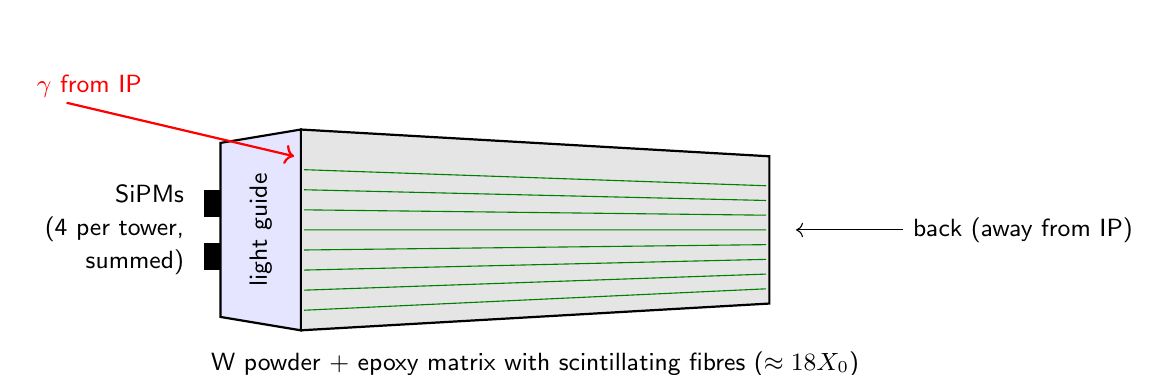
\begin{tikzpicture}[scale=0.85]
\draw[thick,fill=gray!20] (0,0) -- (7,0.4) -- (7,2.6) -- (0,3) -- cycle;
\foreach \y in {0.3,0.6,...,2.7} \draw[green!50!black] (0.05,\y) -- (6.95,{0.4+(\y-0.0)*2.2/3.0-0.0});
\node at (3.5,-0.5) {\small W powder + epoxy matrix with scintillating fibres ($\approx18X_0$)};
\draw[thick,fill=blue!10] (-1.2,0.2) -- (0,0) -- (0,3) -- (-1.2,2.8) -- cycle;
\node[rotate=90] at (-0.6,1.5) {\small light guide};
\fill[black] (-1.45,0.9) rectangle (-1.2,1.3); \fill[black] (-1.45,1.7) rectangle (-1.2,2.1);
\node[anchor=east,align=right] at (-1.6,1.5) {\small SiPMs\\\small (4 per tower,\\\small summed)};
\draw[->,red,thick] (-3.5,3.4) -- (-0.1,2.6) node[pos=0.1,above,red] {\small $\gamma$ from IP};
\draw[->] (9,1.5) -- (7.4,1.5); \node[anchor=west] at (9,1.5) {\small back (away from IP)};
\end{tikzpicture}
\caption{Schematic side view of one EMCal tower: fibres run along the tower, the light exits at the front (towards the IP) through a short light guide onto SiPMs. Not to scale.}\label{fig:block}
\end{figure}

\checksbox{You should be able to reproduce: $24\,576=96\times256$; $6144$ blocks; $0.025\times0.025$ tower size; 64 sectors; one HCal tower above $4\times4$ EMCal towers. If you see 128 or 192 in $i\phi$ in a plot, you are probably looking at the wrong detector or a merged-tower view.}

\pitfallbox{\begin{itemize}
\item The towers are tilted (projective). A shower from a vertex far from $z=0$ enters the towers at an angle, so the shower is wider and the depth of shower maximum maps to a different $\eta$. Vertex-dependent corrections exist for this reason (Module 7).
\item Sector and block boundaries have small dead regions and different response; acceptance maps in $(i\eta,i\phi)$ show this structure.
\end{itemize}}

%=====================================================================
\section{Silicon photomultipliers}\label{sec:sipm}
\goal{Understand the SiPM well enough to explain saturation, temperature dependence, dark noise and radiation damage, all of which appear in sPHENIX calibration and QA.}

\subsection{How a SiPM works}
A SiPM is an array of thousands of tiny avalanche photodiodes (pixels or ``microcells''), all connected in parallel [S09].
Each pixel is reverse-biased \emph{above} its breakdown voltage $V_{\rm bd}$ (Geiger mode).
One photoelectron in a pixel triggers a self-sustaining avalanche, which is stopped (quenched) by a series resistor.
Each fired pixel delivers the same charge $Q=C_{\rm pix}(V_{\rm bias}-V_{\rm bd})$.
The SiPM output is the sum of the fired pixels, so it counts photons.
Key properties:
\begin{itemize}
\item Gain of order $10^5$--$10^6$, so remote digitisation of the signal is possible [S09, S08].
\item Photon detection efficiency (PDE) of about 25\% at the scintillator wavelength [S09].
\item Insensitive to magnetic fields, unlike photomultiplier tubes. This is essential inside a 1.4 T solenoid.
\item Small, cheap and low-power [S08].
\end{itemize}
The EMCal uses Hamamatsu MPPCs with 15 $\mu$m pixels on a $3\times3$ mm$^2$ area [S09, R1], i.e.\ $(3000/15)^2=40\,000$ pixels each.

\subsection{Saturation}
If $N_{\rm pe}$ photoelectrons arrive at a SiPM with $N_{\rm pix}$ pixels spread uniformly and at once, the expected number of fired pixels is
\begin{equation}
N_{\rm fired}=N_{\rm pix}\left[1-\exp\!\left(-\frac{N_{\rm pe}}{N_{\rm pix}}\right)\right]\approx N_{\rm pe}\left(1-\frac{N_{\rm pe}}{2N_{\rm pix}}\right).
\end{equation}
The response is linear only for $N_{\rm pe}\ll N_{\rm pix}$.
If the light illuminates only part of the SiPM (poor light mixing), the effective number of pixels is smaller and saturation sets in earlier [S09].
This is why a two-parameter non-linearity model (light yield and effective pixel number) is used in the sPHENIX simulation of the EMCal response [S15].

\workedbox{size of the saturation effect (toy)}{One tower has $4\times40\,000=160\,000$ pixels. With a toy light yield of 400 p.e./GeV and a 20 GeV photon depositing 80\% of its energy in the central tower, $N_{\rm pe}=6400$. The linear approximation gives a deficit of $N_{\rm pe}/(2N_{\rm pix})=2\%$. If only a quarter of the pixels is effectively illuminated, the deficit becomes about 8\%. Saturation is therefore a percent-level effect at the highest photon energies in sPHENIX and must be in the simulation. (Toy numbers.)}

\subsection{Temperature dependence}
$V_{\rm bd}$ increases with temperature.
At fixed bias, a higher temperature means a smaller overvoltage $V_{\rm bias}-V_{\rm bd}$ and therefore a smaller gain and PDE.
The effect is a few percent per degree Celsius for typical operating overvoltages [S09, S16].
sPHENIX handles it in two ways: the calorimeter electronics are cooled and temperature-monitored, and the HCal calibration includes a run-by-run temperature correction (Section~\ref{sec:calib}) [S16].

\subsection{Dark counts and radiation damage}
Thermal electrons can trigger avalanches without light: these are dark counts, at a rate of order hundreds of kHz per mm$^2$ at room temperature.
Neutrons damage the silicon lattice: an incoming particle knocks a silicon atom out of its site (displacement damage, quantified by the non-ionising energy loss, NIEL), creating defects that generate dark current [S09].
Dark current and dark-count rate grow with neutron fluence, and the recovery (annealing) is slow and small [S09].
For a calorimeter this means a slowly rising pedestal noise, i.e.\ a growing noise term $c/E$ in Eq.~\eqref{eq:res}.
sPHENIX was the first large deployment of SiPMs exposed to a significant neutron fluence in a collider experiment [S09].

\connectbox{Rising SiPM noise over the years raises the pedestal width and therefore the energy below which towers are zero-suppressed or treated as noise.
In your analysis this enters through the minimum cluster energy and the cluster $\chi^2$/probability: if you compare Run-24 with later runs, check that the noise level has not shifted your low-$p_T$ photon efficiency.}

%=====================================================================
\section{Hadronic showers}\label{sec:had}
\goal{Understand why hadronic calorimetry is harder than electromagnetic calorimetry: larger and more fluctuating showers, invisible energy, $e/h\neq1$, leakage.}

\subsection{Nuclear interaction length}
A hadron travels on average one \textbf{nuclear interaction length} $\lambda_I$ before an inelastic nuclear collision.
$\lambda_I$ scales roughly as $A^{1/3}$ and is much longer than $X_0$ for heavy materials: for iron $\lambda_I\approx16.8$ cm while $X_0\approx1.76$ cm; for tungsten $\lambda_I\approx9.9$ cm while $X_0\approx0.35$ cm [R4].
A hadronic calorimeter must therefore be many times deeper than an electromagnetic one.
The sPHENIX EMCal, at about 18 $X_0$, is less than one $\lambda_I$ deep (about 0.7 $\lambda_I$) [S08].
About half of the hadrons start their shower in the EMCal and the rest in the HCal.

\subsection{Composition of a hadronic shower}
In each nuclear interaction the hadron produces secondary pions, nucleons and nuclear fragments.
\begin{itemize}
\item \textbf{Electromagnetic component.} Neutral pions decay immediately to two photons, which shower electromagnetically. Once energy has gone into the EM component it never comes back (a $\pi^0$ does not make hadrons), so the EM fraction $f_{\rm em}$ grows with each generation. A common parametrisation is $f_{\rm em}=1-(E/E_0)^{k-1}$ with $E_0\approx1$ GeV and $k\approx0.82$ for pions [R6]. This gives $f_{\rm em}\approx0.25$ at 5 GeV and $\approx0.46$ at 30 GeV.
\item \textbf{Hadronic component.} Charged hadrons ionise; neutrons travel far and deposit energy late; a sizeable fraction of the energy goes into breaking nuclei (binding energy) and is \emph{invisible}.
\end{itemize}

\subsection{Non-compensation, $e/h$ and $\pi/e$}
Let $e$ be the response to the EM component and $h$ the response to the non-EM component, per unit energy.
Because of invisible energy, typically $h<e$.
The response to a pion relative to an electron of the same energy is
\begin{equation}
\frac{\pi}{e}=f_{\rm em}+(1-f_{\rm em})\frac{h}{e}.
\end{equation}
Since $f_{\rm em}$ rises with energy, $\pi/e$ rises with energy: a non-compensating calorimeter ($e/h\neq1$) is non-linear for hadrons.
Since $f_{\rm em}$ fluctuates event by event, the response fluctuates: this adds a large stochastic term and a constant term to the hadron resolution.
With a toy $h/e=0.6$, $\pi/e$ goes from about 0.70 at 5 GeV to about 0.78 at 30 GeV.
Good hadronic resolution requires $e/h\to1$ (``compensation'') [S09].
sPHENIX does not attempt compensation; the jet energy scale is corrected in software (Module 7).

\subsection{Shower size and containment}
Hadronic showers are long and wide.
Empirical rules [R6]: the depth of maximum is $t_{\max}\approx0.2\ln E[\mathrm{GeV}]+0.7$ (in $\lambda_I$), and 95\% longitudinal containment needs $L_{95}\approx t_{\max}+2.5\,\lambda_{\rm att}$ with $\lambda_{\rm att}\approx\lambda_I(E/\mathrm{GeV})^{0.13}$.

\workedbox{how deep must the sPHENIX calorimeter be?}{For a 20 GeV hadron: $t_{\max}=0.2\times3.0+0.7=1.3\,\lambda_I$; $\lambda_{\rm att}=20^{0.13}=1.48\,\lambda_I$; $L_{95}\approx1.3+3.7=5.0\,\lambda_I$.
For 10 GeV: $4.5\,\lambda_I$; for 50 GeV: $5.6\,\lambda_I$.
The full sPHENIX stack (EMCal $\approx0.7\lambda_I$, inner HCal, solenoid, outer HCal $\approx3.5\lambda_I$) is roughly $5\lambda_I$ [S08, R3].
So it contains about 95\% of a 20 GeV hadron shower on average, and a 50 GeV hadron leaks noticeably. The design target was 95\% containment around 20--30 GeV, and the calorimeters are ``a little thin'' by design, so leakage at high energy is real and must come from simulation [S08].}

\pitfallbox{\begin{itemize}
\item Calling the HCal ``calibrated'' without saying to \emph{what}: sPHENIX calibrates the HCal to the \emph{electromagnetic scale} (Section~\ref{sec:calib}). A hadron then reads low by $\pi/e<1$, and the jet energy scale correction restores it.
\item The three longitudinal compartments are made of different materials (tungsten EMCal, aluminium inner HCal, steel outer HCal), each with its own $e/h$ and sampling fraction [S08]. A hadron's measured energy depends on where it starts showering.
\end{itemize}}

%=====================================================================
\section{The sPHENIX HCal}\label{sec:hcal}
\goal{Know the geometry and construction of the inner and outer HCal and the reasons for the tilted-plate design.}

\subsection{Overview}
The HCal is the first mid-rapidity sampling hadronic calorimeter at RHIC [S16].
It has two layers:
\begin{itemize}
\item \textbf{Inner HCal (iHCal):} inside the solenoid, directly behind the EMCal, at a radius of roughly 1.2--1.4 m. Its absorber is mostly aluminium; it also serves as the support frame for the EMCal [S08].
\item \textbf{Outer HCal (oHCal):} outside the solenoid, at a radius of roughly 1.9--2.6 m. Its absorber is tapered low-carbon steel plates which are also the magnet flux return [S08].
\end{itemize}
Each layer has $24\times64$ towers in $\eta\times\phi$, i.e.\ 1536 towers, with $\Delta\eta\times\Delta\phi\approx0.1\times0.1$, covering $|\eta|<1.1$ and $2\pi$ [S08, S16].
Each layer is built from 32 sectors in $\phi$; one sector is 2 towers wide in $\phi$ and 24 towers long in $\eta$ [S16].

\subsection{Tiles, fibres and SiPMs}
The active medium consists of extruded plastic scintillator tiles with an embedded wavelength-shifting (WLS) fibre in a groove [S08, S16].
The WLS fibre absorbs the blue scintillation light and re-emits it at a longer wavelength, which is trapped and guided to one end of the fibre, where a $3\times3$ mm$^2$ SiPM reads it out [S08].
Each tower combines the signals of several tiles in depth: 5 tiles per tower in the oHCal and 4 in the iHCal [S16].
In total there are $1536\times5=7680$ tiles/SiPMs in the oHCal and $1536\times4=6144$ in the iHCal [S16].
The tile shapes vary with $\eta$ (projective geometry), so there are many different tile types; tile production and quality control (light yield, uniformity) were a large part of the project [S08].
The response across each tile was \emph{mapped} with beam at Fermilab, and rules of thumb for the fibre routing were developed to make the light collection as uniform as possible [S08].

\subsection{Why tilted plates?}
In a plain radial geometry, a particle from the vertex could travel along a gap between plates and never sample the active medium (``channelling'').
Tilting the plates with respect to the radial direction means that every straight track from the vertex crosses several plates and tiles [S08].
The tilt also lets the plates double as an efficient magnetic flux return [S08].
Two side effects had to be studied: a small asymmetry between positively and negatively charged particles (which bend in opposite directions in $\phi$ and therefore cross the tilted plates at different angles), and a sampling fraction that changes with depth [S08].

\begin{figure}[h]\centering
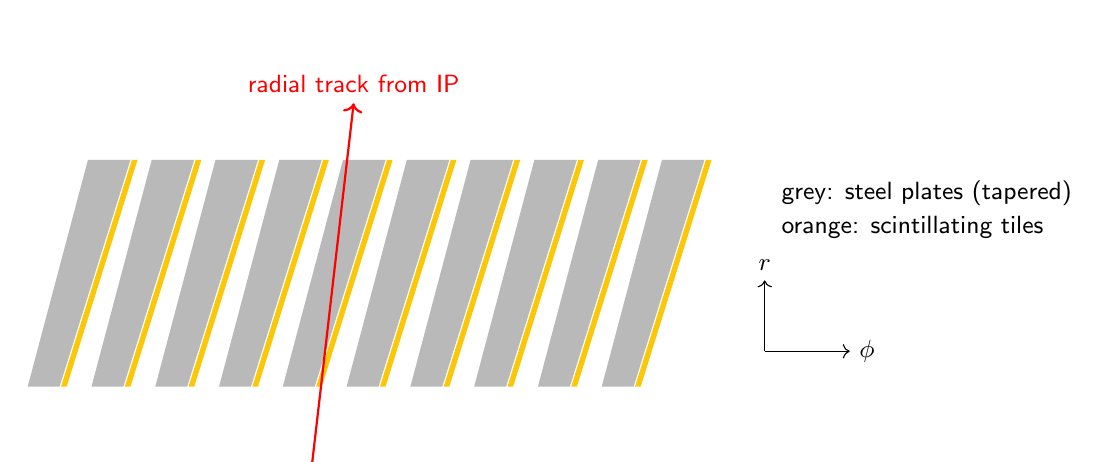
\begin{tikzpicture}[scale=0.9]
\foreach \k in {0,...,9}{
 \pgfmathsetmacro{\x}{\k*0.9}
 \fill[gray!55] (\x,0) -- (\x+0.45,0) -- (\x+1.45,3.2) -- (\x+0.85,3.2) -- cycle;
 \fill[yellow!60!orange] (\x+0.47,0) -- (\x+0.55,0) -- (\x+1.55,3.2) -- (\x+1.47,3.2) -- cycle;
}
\draw[->,red,thick] (4.0,-1.2) -- (4.6,4.0) node[above,red] {\small radial track from IP};
\node[anchor=west,align=left] at (10.5,2.5) {\small grey: steel plates (tapered)\\ \small orange: scintillating tiles};
\draw[->] (10.4,0.5) -- (11.6,0.5) node[right] {\small $\phi$};
\draw[->] (10.4,0.5) -- (10.4,1.5) node[above] {\small $r$};
\end{tikzpicture}
\caption{Schematic of the tilted-plate HCal in the $r$--$\phi$ plane: a radial track always crosses several absorber plates and tiles. Not to scale; tilt angle exaggerated.}\label{fig:tilt}
\end{figure}

\subsection{Depth budget}
Approximate depths along a radial line at $\eta=0$ [S08]:
\begin{center}\begin{tabular}{@{}lll@{}}\toprule
Element & Material & Depth\\\midrule
EMCal & W powder/epoxy + fibres & $\approx18X_0\approx0.7\lambda_I$\\
Inner HCal & mostly aluminium + tiles & small fraction of $\lambda_I$\\
Solenoid & superconducting coil, cryostat & $\approx1.4X_0$\\
Outer HCal & steel + tiles & $\approx3.5\lambda_I$\\\bottomrule
\end{tabular}\end{center}
The original inner HCal design used steel; the as-built inner HCal is an aluminium frame [S08, S47].
This matters for comparing with the 2016--2018 beam tests, which had a steel inner HCal (Section~\ref{sec:tb}).

\subsection{The LED system}
Each HCal channel can be flashed with an LED.
The original hope was to track gains with LEDs alone [S08].
In practice the coupling of the LED to each tile is variable, the light is injected at a single point close to the SiPM (so it does not sample the tile response), the LED pulser stability itself must be characterised, and in the oHCal the LED signals of the five tiles of a tower are summed [S08].
LEDs are therefore excellent for channel checks, timing and \emph{relative} gain changes (e.g.\ the temperature coefficient), but not for the absolute energy scale.
The absolute scale comes from physics signals: cosmic muons and collision data (Section~\ref{sec:calib}).

\checksbox{$1536=24\times64$ towers per layer; $0.1\times0.1$; 32 sectors per layer; 5 tiles/tower in oHCal, 4 in iHCal. One HCal tower $\leftrightarrow$ $4\times4$ EMCal towers. In a tower-occupancy map, look for the sector structure every 2 towers in $i\phi$ and for special regions near support structures and the ``chimney'' (where the magnet services exit) [S16].}

\connectbox{Your analysis does not use the HCal energy directly, but it touches it in two ways.
(1) Photon isolation and some photon-ID variables use the HCal energy behind the EMCal cluster: hadrons and merged $\pi^0$s can leave energy in the iHCal.
(2) The jet triggers combine EMCal and HCal energy; if you look at Jet-trigger samples for cross-checks, the HCal calibration enters through the trigger threshold.}

%=====================================================================
\section{Readout chain: from light to a calibrated tower}\label{sec:readout}
\goal{Follow one tower signal from the SiPM to the \code{TowerInfo} object in your DST, and know which quantities you can trust.}

\subsection{Front end and digitisation}
\begin{enumerate}
\item The SiPM signal is amplified and shaped by a preamplifier close to the detector. The EMCal readout boards are mounted with the SiPMs on the sector; the HCal uses similar SiPM preamplifier boards [S09, S08].
\item The analog signals travel to digitiser crates in racks on the detector platform. Large SiPM signals made remote digitisation possible [S08].
\item Each channel is sampled by a 14-bit flash ADC at six times the RHIC beam clock, about 56 MHz [S08, S15]. The RHIC bunch spacing is about 106 ns ($1/(78.2\ \mathrm{kHz}\times120)$ buckets), so one sample is about 17.7 ns, and a pulse spans several samples.
\item On a trigger (Module 5), a short window of samples is read out per channel (16 samples in the 2024--2026 runs [S15]).
\end{enumerate}

\subsection{Zero suppression}
Most towers in a $p$+$p$ event see no signal.
To save bandwidth, a channel is \emph{zero suppressed}: only two samples are kept (an early, pre-pulse sample and the sample at the expected peak), unless the difference between them exceeds a threshold, in which case the full waveform is kept [S15].
For a zero-suppressed channel the energy estimate is just the difference of the two samples, and time and $\chi^2$ are undefined [S15].

\subsection{Waveform fitting}
For full waveforms, the offline module \code{CaloTowerBuilder} (coresoftware \code{offline/packages/CaloReco}) fits a template pulse shape to the samples [S15].
The fit returns:
\begin{itemize}
\item the \textbf{amplitude} (peak height above pedestal, in ADC counts);
\item the \textbf{peak time} (in units of samples);
\item the \textbf{pedestal};
\item a \textbf{fit-quality} $\chi^2$ per degree of freedom;
\item an 8-bit \textbf{status} word.
\end{itemize}
These ``distilled'' tower quantities are written to the production DSTs as a \code{TowerInfo} container (node \code{TOWERS\_CEMC} for the EMCal; similar nodes for the HCal and sEPD) [S15].
The tower values in the DST are \emph{uncalibrated}, in ADC counts [S15].
Several \code{TowerInfo} versions exist (v1 saves only the energy; later versions add time, $\chi^2$, pedestal and, optionally, the waveform); the DSTs use a compact version with reduced precision for time and $\chi^2$ [S15]. Check the current coresoftware source for the exact layout.

\begin{figure}[h]\centering
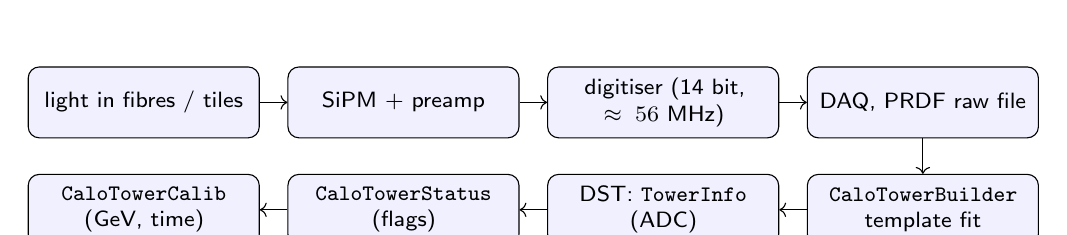
\begin{tikzpicture}[node distance=0.45cm and 0.35cm, box/.style={draw,rounded corners,fill=blue!6,align=center,font=\footnotesize,minimum height=0.9cm,text width=2.7cm}]
\node[box] (a) {light in fibres / tiles};
\node[box,right=of a] (b) {SiPM + preamp};
\node[box,right=of b] (c) {digitiser (14 bit, $\approx56$ MHz)};
\node[box,right=of c] (d) {DAQ, PRDF raw file};
\node[box,below=of d] (e) {\code{CaloTowerBuilder} template fit};
\node[box,left=of e] (f) {DST: \code{TowerInfo} (ADC)};
\node[box,left=of f] (g) {\code{CaloTowerStatus} (flags)};
\node[box,left=of g] (h) {\code{CaloTowerCalib} (GeV, time)};
\draw[->] (a)--(b); \draw[->] (b)--(c); \draw[->] (c)--(d); \draw[->] (d)--(e); \draw[->] (e)--(f); \draw[->] (f)--(g); \draw[->] (g)--(h);
\end{tikzpicture}
\caption{Schematic calorimeter signal chain. The top row is hardware (Modules 3 and 5); the bottom row is software (Modules 6 and 7). Status and calibration are applied when you run the calorimeter reconstruction macro on the DST [S15].}\label{fig:chain}
\end{figure}

\subsection{Status flags and calibration on the fly}
When you run the standard calorimeter macro (\code{Process\_Calo} in the macros repository) on a DST, two modules run [S15]:
\begin{itemize}
\item \code{CaloTowerStatus} sets per-tower flags, for example: hot/dead/cold (from an offline comparison of towers at the same $\eta$, with $5\sigma$ outliers flagged), bad $\chi^2$, not instrumented, no calibration available, zero suppressed, saturated (the waveform reached the ADC maximum) [S15].
\item \code{CaloTowerCalib} multiplies each tower amplitude by a single calibration constant (separate constants for zero-suppressed and full-waveform amplitudes) to convert ADC to GeV, and subtracts the run-averaged tower time so that calibrated times are centred near zero [S15].
\end{itemize}
The constants come from the conditions database (CDB) through \code{CDBInterface}, selected by a global tag and the run number (Module 6).
In the EMCal, ``GeV'' is defined such that a single photon has a response of 1, i.e.\ it is a photon energy scale [S15].

\pitfallbox{\begin{itemize}
\item Using the DST \code{TOWERS\_CEMC} values directly as energies: they are ADC counts. Use the calibrated node produced by the macro (in your analysis, \code{TOWERINFO\_CALIB\_CEMC}).
\item Ignoring the status word: hot towers make fake high-$p_T$ clusters; bad-$\chi^2$ towers have distorted pulses (e.g.\ pile-up or electronics problems) [S15].
\item Mixing zero-suppressed and full-waveform towers without care: their energy estimators differ (two-sample difference vs.\ template amplitude), and they have separate calibration constants [S15].
\item Timing is reported in samples, not ns, and has an energy dependence that is not fully understood [S15].
\end{itemize}}

%=====================================================================
\section{Test beams and simulation}\label{sec:tb}
\goal{Know what the test beams established, how to read their results critically, and why simulation is the bridge from test beam to sPHENIX.}

\subsection{The test-beam campaigns}
Prototypes were tested at the Fermilab Test Beam Facility as experiment T-1044 [S09, S08, S47, R1, R2]:
\begin{itemize}
\item 2014: proof-of-principle prototypes.
\item 2016: prototypes at $\eta\approx0$ (EMCal + inner HCal + outer HCal in all combinations; the inner HCal was steel). Published in [R1].
\item 2017: prototypes at $\eta\approx0.9$ (high-$\eta$ geometry).
\item 2018: improved high-$\eta$ EMCal blocks (a 2D-projective prototype built like a real sector in mechanics, electronics and cooling) [S09]; EMCal results published in [R2]. Some data were also taken with an uninstrumented aluminium inner-HCal frame [S47].
\end{itemize}
Beam energies ranged up to about 30 GeV, with mixed electron/hadron beams; Cherenkov counters tagged electrons, and wire chambers or hodoscopes measured the beam position [R1].

\subsection{Combining compartments}
In a test beam with several longitudinal compartments, the hadron energy is reconstructed as a weighted sum, for example $E=c\,[g\,E_{\rm EMCal}+w\,E_{\rm iHCal}+E_{\rm oHCal}]$.
The weights correct for different sampling fractions and $e/h$ in each compartment.
In the published 2016 analysis the inner-HCal signal was given a larger weight than the outer-HCal signal in data, and the EMCal weight was tuned versus the EMCal energy fraction to flatten the response [S47, R1].

\subsection{Lessons from re-analysing the test beam}
A 2026 workfest study re-ran the original prototype Geant4 simulation (code in the public sPHENIX \code{prototype} repository) to compare data and simulation in a way that could constrain the single-hadron energy scale used in jet calibrations [S47].
The general lessons, which apply to any test-beam or calibration plot you read:
\begin{enumerate}
\item Check the normalisation. If each energy point is scaled to the beam energy separately, only widths are compared, not linearity or absolute scale.
\item Check that the geometry in the simulation matches the hardware that was in the beam (there were two different steel inner-HCal prototypes, and a mismatch was found and fixed by comparing Geant4 hit files) [S47].
\item Check the beam composition at low energy: muon or other contamination can bias the low-energy points [S47].
\item Weights must be the same in data and simulation for an apples-to-apples comparison [S47].
\item The final sPHENIX inner HCal is aluminium, not steel. Leakage differs from the prototype, so the full sPHENIX geometry must be simulated and the leakage modelling varied as a systematic [S47].
\end{enumerate}

\subsection{Simulation in sPHENIX}
The full detector is simulated with Geant4 inside Fun4All through \code{PHG4Reco} (Module 6).
The calorimeter geometries are set up in the standard macros (in the \code{macros} repository, \code{common/} directory, e.g.\ \code{G4\_CEmc\_Spacal.C}, \code{G4\_HcalIn\_ref.C}, \code{G4\_HcalOut\_ref.C}; check the current names).
Geant4 deposits are converted to light (with the sampling structure and, for the EMCal, a light-collection map), then to waveforms that mimic the real electronics, so that the same \code{CaloTowerBuilder} reconstruction runs on data and simulation.
EMCal SiPM non-linearity was included in the test-beam simulation and a two-parameter model has been implemented for sPHENIX simulation; samples must be re-digitised to include it [S15].

\connectbox{Your efficiency uses PYTHIA8 events through the sPHENIX simulation plus extra EMCal smearing tuned on data.
Three hardware effects in this module must be correctly in that simulation or covered by systematics: (1) lateral and longitudinal leakage (energy scale per cluster); (2) SiPM non-linearity (high-$p_T$ photons); (3) the dead/hot tower map (acceptance). For (3) the simulation should use the same tower-status map as the data, or you should apply the data map to the simulated towers.}

%=====================================================================
\section{Calibration strategy overview}\label{sec:calib}
\goal{Understand the logic of the calibration chain for both calorimeters: what each step fixes, what physics it relies on, and what it cannot fix. The details of the code are in Module 7.}

\subsection{What a calibration must do}
For each tower $i$ we need a constant $k_i$ such that $E_i=k_i\,A_i$, where $A_i$ is the amplitude in ADC counts.
It is useful to split $k_i=K\cdot r_i(t)$:
\begin{itemize}
\item an \textbf{absolute scale} $K$ (common to all towers, or to all towers at a given $\eta$), which makes the energy correct on average;
\item a \textbf{relative} (inter-tower) factor $r_i$, which equalises towers;
\item a \textbf{time dependence} $r_i(t)$, from temperature, radiation damage and hardware changes.
\end{itemize}
Errors in $r_i$ broaden peaks (they enter the constant term $b$); errors in $K$ shift peaks and spectra.

\subsection{Tools available}
\begin{center}\small
\begin{tabularx}{\linewidth}{@{}lXX@{}}\toprule
Tool & What it measures & Limitations\\\midrule
Test beam & absolute response, resolution, linearity for prototypes & different hardware and environment\\
LED & channel alive, timing, relative gain changes & no absolute scale; coupling varies [S08]\\
Cosmic muons (MIP) & energy deposit of a known particle in each tower & must be converted to the shower scale with simulation; muons are mostly vertical [S16]\\
Tower slope & relative gain from the shape of each tower's energy spectrum in beam data & needs symmetry (all towers at one $\eta$ see the same spectrum) [S42, S16]\\
$\pi^0\to\gamma\gamma$ & absolute photon scale and tower-by-tower gains (EMCal) & needs statistics, depends on resolution and non-linearity [S15]\\
Isolated hadrons, $E/p$ & hadron response with tracks & needs tracking; planned [S16]\\\bottomrule
\end{tabularx}\end{center}

\subsection{The tower-slope method}
\textbf{Idea.} In minimum-bias data, all towers at the same $\eta$ should see the same energy spectrum, because the physics is symmetric in $\phi$.
If tower $i$ has a gain $g_i$ relative to the average, its spectrum is a stretched copy of the reference.

\textbf{Derivation.} Let the true spectrum be $F(E)$. The measured spectrum of tower $i$ is
\begin{equation}
f_i(E')=\frac{1}{g_i}F\!\left(\frac{E'}{g_i}\right),\qquad E'=g_iE .
\end{equation}
For a locally exponential spectrum $F(E)\propto e^{-E/T}$, $f_i(E')\propto e^{-E'/(g_iT)}$: the gain simply multiplies the inverse slope.
So the ratio of fitted slopes gives $g_i$ directly.
In practice the reference is the sum of all tower spectra in the same $\eta$ ring, and a two-parameter function (normalisation and gain stretch) built from the reference is fitted to each tower's spectrum [S42, S16].
The low-energy region is excluded, because noise, pedestal fluctuations, zero suppression and trigger thresholds distort it [S42].

\textbf{Why it is useful.} It needs no special run and no reconstruction beyond towers. It is applied as a relative correction on top of an absolute calibration (cosmics in the HCal), so it should leave the overall scale unchanged; a check that the averaged correction preserves the absolute scale is part of the validation [S42].

\textbf{Where it fails.} Towers where the $\phi$ symmetry is broken by material: support structures and the chimney region. These are excluded from the method [S16].

\conceptbox{Link to your M.S. work}{Your Tower Slope calibration MC studies tested exactly this method for the EMCal: inject known gain offsets in simulation, run the slope fits, and check how well the injected $g_i$ are recovered as a function of statistics and fit range. The two lessons from Section~\ref{sec:calib}---exclude the low-energy region and respect the symmetry assumption---are the same ones you met there.}

\subsection{HCal: cosmics, tower slope, temperature, special cases}
The HCal calibration has four steps [S16]:
\begin{enumerate}
\item \textbf{Absolute scale from cosmic muons.} Dedicated cosmic runs select muons that pass vertically through a whole tower (topological cuts using neighbouring towers). The deposited-energy spectrum of each tower is fitted (a gamma-type function) to find its most probable value (MPV) in ADC. The same is done in a cosmic-muon simulation, giving the MPV in MeV. The ratio converts ADC to energy at the \emph{electromagnetic} scale, tower by tower.
\item \textbf{Relative correction by tower slope} with beam data (above), for effects not in the cosmic simulation (e.g.\ structures outside the main detector body).
\item \textbf{Run-by-run temperature correction}, using the SiPM gain temperature coefficient (measured with LEDs) and the recorded temperature, to transport the cosmic calibration to each physics run.
\item \textbf{Special corrections} for rare, correctable channel pathologies, e.g.\ a tower whose signal is halved or doubled for a period because of a cable connection problem; these are found by inspecting per-tower hit rates versus run number.
\end{enumerate}
\textbf{Validation.} The calibration stability is checked with the hit rate per tower per event versus time. Because this rate grows with the probability of a second collision in the same crossing, it must be corrected for pile-up [S16].

\workedbox{pile-up probability per crossing}{RHIC revolution frequency $\approx78$ kHz; with 111 filled bunches per ring, colliding crossings occur at $f_{\rm bc}\approx8.7$ MHz [S16].
For an interaction rate $R$, the mean number of collisions per crossing is $\mu=R/f_{\rm bc}$, and for Poisson statistics the probability of two or more collisions given at least one is
$P(\ge2|\ge1)=[1-e^{-\mu}(1+\mu)]/(1-e^{-\mu})\approx\mu/2$.
Toy rates: $R=10$ kHz gives $\mu=0.0012$ and $P\approx0.06\%$; $R=300$ kHz gives $\mu=0.035$ and $P\approx1.7\%$.
The rate-dependent part of the hit rate must be removed before using it as a gain monitor. In practice a data-driven correction may work better than the simple Poisson formula [S16]. (Toy rates.)}

\subsection{EMCal: $\pi^0$ gain balancing and absolute scale}
The EMCal calibration uses the $\pi^0\to\gamma\gamma$ peak [S15]:
\begin{enumerate}
\item \textbf{Start} from an initial set of constants (from lab tests, cosmics, or a previous calibration).
\item \textbf{Gain balancing.} For each tower, fill the diphoton mass spectrum for pairs where one cluster's leading tower is that tower. Fit the $\pi^0$ peak. Correct the tower gain by the ratio of the target to the fitted mass. Iterate, because changing one tower's gain changes clusters that share it with neighbours.
\item \textbf{Absolute scale.} Match the peak position to simulation, not to the PDG mass, because the reconstructed peak is shifted by resolution, leakage, the clustering and the kinematic selection. The absolute scale is sensitive to the single-photon resolution, so the MC cluster energies and positions are smeared until the data and MC $\pi^0$ and $\eta$ peaks agree [S15].
\item \textbf{Timing calibration.} Subtract each tower's mean time so that prompt photons sit at zero; the photon timing resolution can be checked with the time difference of the two $\pi^0$ decay photons [S15].
\item \textbf{Non-linearity.} Model the SiPM and electronics non-linearity in simulation (two-parameter model) [S15].
\end{enumerate}
The tower-slope method can also be used for the EMCal as a fast relative calibration or a starting point.

\workedbox{why the peak is not at 135 MeV}{Suppose each photon's measured energy is $E'=(1-\ell)E$, with leakage $\ell=5\%$ not absorbed in the calibration. Then $m'=\sqrt{2E_1'E_2'(1-\cos\theta)}=(1-\ell)m$, and the peak moves to about 128 MeV. Now add resolution: a falling $p_T$ spectrum feeds more low-energy pairs upward into a fixed $p_T$ bin than the reverse, so pairs that fluctuated up in energy are over-represented, and the peak in a given $p_T$ bin moves \emph{up}. The two effects partly cancel, by an amount that depends on $p_T$. Hence the calibration target is ``peak position in data equals peak position in MC'', not ``peak equals the PDG mass''. (Toy reasoning.)}

\checksbox{\begin{itemize}
\item After calibration, the tower-by-tower $\pi^0$ peak positions should scatter much less than before; their spread is a direct estimate of the remaining relative miscalibration.
\item A tower-occupancy map at fixed $\eta$ should be flat in $\phi$ except for known structures.
\item The hit rate per event versus run (pile-up corrected) should be flat after the temperature correction.
\item The calibrated time of prompt clusters should peak at zero.
\end{itemize}}

\pitfallbox{\begin{itemize}
\item Calibrating relative gains with the tower-slope method in a region where $\phi$ symmetry is broken (supports, chimney, sector edges with dead neighbours).
\item Using a trigger-selected sample for the tower slope: the trigger threshold biases the spectrum shape tower by tower. Use minimum-bias data or fit only far above threshold.
\item Calibrating the $\pi^0$ peak to the PDG mass in data and also in MC with different procedures: the data/MC energy scale is then inconsistent.
\item Forgetting the time dependence: a calibration from one period applied to another period without temperature/run corrections.
\end{itemize}}

\connectbox{\begin{itemize}
\item The global tag and the calibration version used for \code{DST\_CALOFITTING}-based reconstruction must be the same for all runs in your cross section, or you must show the difference is negligible.
\item The residual tower-to-tower miscalibration enters your $\pi^0$ width (constant term). It is one of the reasons the MC smearing is needed.
\item The Photon triggers (bits 29 and 30 in your run period) fire on EMCal energy sums computed from \emph{online} tower energies with \emph{online} gains; their turn-on curves in offline energy are therefore smeared by the offline/online calibration difference (Module 5).
\end{itemize}}

%=====================================================================
\section{Summary}
\begin{itemize}
\item EM showers scale with $X_0$ (depth) and $R_M$ (width); the sPHENIX EMCal has $X_0\approx7$ mm, $R_M\approx2.3$ cm and $\approx18X_0$ depth, and a 2 GeV photon is about 91\% contained in a $3\times3$ array (toy estimate).
\item The EMCal is a W-powder/epoxy SPACAL with 0.47 mm fibres, $f_{\rm samp}\approx2\%$, $96\times256$ projective towers read out by four SiPMs each; the sampling term alone gives about $13\%/\sqrt{E}$.
\item The HCal has two layers of $24\times64$ towers ($0.1\times0.1$): aluminium inner HCal inside the solenoid and steel outer HCal (the flux return) outside, both with tilted plates and tile+WLS+SiPM readout.
\item Public beam-test resolutions: EMCal $2.8\%\oplus15.5\%/\sqrt{E}$ at $\eta\approx0$; hadrons in EMCal+HCal $13.5\%\oplus64.9\%/\sqrt{E}$.
\item Signals are digitised at six times the beam clock, fitted offline by \code{CaloTowerBuilder}, written as uncalibrated \code{TowerInfo}, and flagged/calibrated on the fly by \code{CaloTowerStatus} and \code{CaloTowerCalib}.
\item Calibration: cosmics (HCal absolute), tower slope (relative), temperature (time), $\pi^0$ (EMCal relative and absolute), with MC smearing tuned to data.
\end{itemize}

%=====================================================================
\section{Hands-on exercises on SDCC (optional, suggested)}
These exercises are optional. They have not been run as part of writing this module; commands and names are suggestions that you should check against the current software. The text above does not depend on them.
\begin{enumerate}
\item \textbf{Draw the EMCal tower grid.} On paper or in ROOT, draw a $96\times256$ \code{TH2} in $(i\eta,i\phi)$; overlay block boundaries every 2 towers, sector boundaries every 8 towers in $i\phi$ and at $i\eta=48$, and the $24\times64$ HCal grid. Convert tower indices to $\eta$ and $\phi$ by $\eta\approx-1.1+(i\eta+0.5)\times2.2/96$ and $\phi=(i\phi+0.5)\times2\pi/256$ (approximate; the real geometry is in the geometry node).
\item \textbf{Containment calculator.} Write a 20-line Python or ROOT script that evaluates $P(a,bT)$ for the gamma profile and reproduces the containment numbers of Section~\ref{sec:em} for $E=0.5$--30 GeV. Then vary $E_c$ from 8 to 12 MeV to see how sensitive the estimate is.
\item \textbf{Tower map from a DST.} Set up the environment, take one \code{DST\_CALOFITTING} file of a Run-24 $p$+$p$ run from the FileCatalog (Module 5), run \code{Process\_Calo()}, and in a small \code{SubsysReco} loop over \code{TOWERINFO\_CALIB\_CEMC} fill an occupancy map for towers above 0.5 GeV and a map of towers flagged hot. Identify the sector boundaries. Environment set-up (suggested):
\begin{verbatim}
source /opt/sphenix/core/bin/sphenix_setup.sh -n new
\end{verbatim}
\item \textbf{Look up one tower's calibration in the CDB (checkpoint).} In a ROOT macro, set the global tag and run number through \code{recoConsts} (flags \code{CDB\_GLOBALTAG} and \code{TIMESTAMP}), get the payload URL from \code{CDBInterface}, open it with \code{CDBTTree}, call \code{LoadCalibrations()}, and read the value for one tower key (encode the key with \code{TowerInfoDefs}). A sketch (check the current calibration names and key encoding in coresoftware before running):
{\footnotesize\begin{verbatim}
std::string url = CDBInterface::instance()->getUrl("CEMC_calib_ADC_to_ETower");
CDBTTree *t = new CDBTTree(url);
t->LoadCalibrations();
unsigned int key = TowerInfoDefs::encode_emcal(ieta, iphi);
float k = t->GetFloatValue(key, "CEMC_calib_ADC_to_ETower");
\end{verbatim}}
\item \textbf{Tower-slope toy.} Generate exponential spectra for 256 toy towers with random gains of a few percent, fit each against the summed reference above a threshold, and plot recovered vs.\ injected gain. Repeat with a threshold bias to see the pitfall.
\end{enumerate}

%=====================================================================
\section{Self-test questions}
\begin{enumerate}
\item Why do photons reach shower maximum about one radiation length later than electrons?
\item Estimate $t_{\max}$ for a 10 GeV photon in the sPHENIX EMCal, and the fraction of energy leaking out of an 18 $X_0$ deep block.
\item Why must the EMCal be dense and finely segmented for Au+Au physics? Give a quantitative argument.
\item What is the sampling fraction of the EMCal, and why is it smaller for EM showers than the MIP value?
\item Using the rule of thumb, estimate the stochastic term of a sampling calorimeter with 1 mm fibres and 5\% sampling fraction. Is it better or worse than sPHENIX?
\item For $\sigma_E/E=2.8\%\oplus15.5\%/\sqrt{E}$, at which energy are the stochastic and constant terms equal?
\item Explain SiPM saturation and how it affects a high-energy photon. Why does poor light mixing make it worse?
\item What happens to a SiPM's gain when the temperature rises at fixed bias, and how does sPHENIX correct for it in the HCal?
\item Why is a non-compensating calorimeter non-linear for hadrons?
\item Why are the HCal plates tilted? Name one side effect that had to be studied.
\item A DST tower in \code{TOWERS\_CEMC} has amplitude 250. What energy is that, and what do you need to know to convert it?
\item What is a zero-suppressed tower, and what are its energy, time and $\chi^2$?
\item State the assumption behind the tower-slope method and two places in the HCal where it fails.
\item Why is the EMCal absolute scale tuned by matching the $\pi^0$ peak to MC rather than to 135 MeV?
\item Why can LEDs not provide the absolute HCal scale?
\end{enumerate}

\appendix
\section{Answers}
\begin{enumerate}
\item A photon must first convert into an $e^+e^-$ pair, with mean free path $\tfrac97X_0$; until then nothing is deposited. Electrons start radiating immediately. The parametrisation encodes this as $C_\gamma-C_e=+1$.
\item $t_{\max}=\ln(10000/8)+0.5=7.1+0.5\approx7.6\,X_0$ (about 5.3 cm). With $b=0.5$, $a=1+0.5\times7.6=4.8$, and $P(4.8,9)\approx0.95$, so about 5\% leaks out of the back (pure-tungsten $E_c$; somewhat less for the real mixture).
\item The underlying event deposits energy in every tower. Its contribution to a cluster scales with the cluster area. With $\mathrm{d}E_T/\mathrm{d}\eta\sim600$ GeV, a $3\times3$ array ($\approx0.0055$ in $\eta\phi$) collects $\sim0.5$ GeV, comparable to the 0.34 GeV resolution for a 5 GeV electron. A larger $R_M$ or larger towers would make the UE dominate. Density (small $X_0$ and $R_M$) also lets the calorimeter fit into 26 cm of radius.
\item About 2\%. Soft photons in the shower are absorbed preferentially by the high-$Z$ tungsten (photoelectric cross section $\propto Z^{4-5}$), so the active fibres see less than their MIP share.
\item $2.7\%\sqrt{1/0.05}=2.7\%\times4.47=12\%$. Slightly better than the sPHENIX $\approx13\%$, but such a calorimeter would be less dense (more active material) and so need more space.
\item $15.5\%/\sqrt{E}=2.8\%$ gives $\sqrt{E}=5.5$, $E\approx31$ GeV.
\item Each SiPM pixel fires at most once per pulse, so the number of fired pixels is $N_{\rm pix}(1-e^{-N_{\rm pe}/N_{\rm pix}})$ and falls below $N_{\rm pe}$ as the light grows. A high-energy photon concentrates light in one tower, so its energy is underestimated. With poor mixing only part of the pixel area is illuminated, the effective $N_{\rm pix}$ is smaller, and saturation starts at lower energy.
\item The breakdown voltage rises, so the overvoltage, gain and PDE fall (a few percent per degree). The HCal calibration applies a run-by-run correction using the measured temperature and the LED-measured temperature coefficient, relative to the conditions of the cosmic calibration.
\item The EM fraction $f_{\rm em}$ of a hadron shower grows with energy, and the EM and hadronic components have different responses ($e/h\neq1$). So $\pi/e=f_{\rm em}+(1-f_{\rm em})h/e$ grows with energy: the response per GeV changes with energy.
\item So that every straight track from the vertex crosses several absorber plates and tiles (no channelling along gaps), and so that the steel can act as the flux return. Side effects: a charge-dependent ($\pm$) response because positive and negative tracks bend differently relative to the tilt; and a depth-dependent sampling fraction.
\item Nothing yet: it is 250 ADC counts above pedestal. You need the tower's calibration constant for the run (from the CDB via the global tag and run number), applied by \code{CaloTowerCalib}, plus its status (hot, bad $\chi^2$, etc.). You also need to know whether it was zero suppressed, since that uses a separate constant.
\item A channel whose signal was below threshold, so only two samples were kept. Its energy is the difference of the two samples; time and $\chi^2$ are not defined (NaN).
\item All towers at the same $\eta$ see the same energy spectrum ($\phi$ symmetry). It fails near support structures and in the chimney region, where extra material changes the spectrum.
\item The reconstructed peak position is shifted by leakage, clustering, resolution and the kinematic selection in a falling spectrum. Matching data to MC, with MC smeared to the data resolution, makes the data and MC energy scales consistent, which is what an efficiency correction needs.
\item The LED light is injected at one point near the SiPM and does not sample the tile response; its coupling varies from channel to channel; and the LED pulse amplitude itself is not an absolute standard. LEDs measure relative changes well, not energy.
\end{enumerate}

%=====================================================================
\section{Glossary}
\begin{description}[itemsep=1pt,font=\normalfont\bfseries]
\item[Radiation length $X_0$] Distance over which an electron loses $1-1/e$ of its energy by bremsstrahlung; $\tfrac79$ of the photon pair-production mean free path.
\item[Critical energy $E_c$] Energy at which ionisation and radiation losses of electrons are equal; ends shower multiplication.
\item[Moli\`ere radius $R_M$] Transverse shower scale; $\approx90\%$ of the energy lies within $1R_M$.
\item[Nuclear interaction length $\lambda_I$] Mean free path for an inelastic nuclear interaction.
\item[Sampling fraction] Fraction of deposited energy that lands in the active medium.
\item[Stochastic/constant/noise term] The $a/\sqrt{E}$, $b$ and $c/E$ terms of the resolution.
\item[SPACAL] Spaghetti calorimeter: scintillating fibres in an absorber.
\item[Projective tower] Tower whose axis points to the interaction point.
\item[SiPM / MPPC] Silicon photomultiplier, an array of Geiger-mode avalanche photodiodes.
\item[PDE] Photon detection efficiency.
\item[Breakdown voltage] Bias above which a pixel avalanches; rises with temperature.
\item[WLS fibre] Wavelength-shifting fibre that collects tile light and guides it to the SiPM.
\item[$e/h$, $\pi/e$] Ratio of electromagnetic to hadronic response; pion-to-electron response ratio.
\item[Zero suppression] Keeping only two samples for a channel below threshold.
\item[Template fit] Fit of a reference pulse shape to the waveform samples.
\item[\code{TowerInfo}] The tower object (energy, time, $\chi^2$, status) in sPHENIX DSTs.
\item[Tower slope] Relative calibration from the shape of each tower's spectrum, assuming $\phi$ symmetry.
\item[MIP / MPV] Minimum-ionising particle / most probable value of its deposit.
\item[CDB, global tag] Conditions database and the label that selects a consistent set of calibrations.
\item[Chimney] Region of the detector where the magnet services exit; non-standard material.
\end{description}

%=====================================================================
\section*{References}
\addcontentsline{toc}{section}{References}
\subsection*{School talks (sPHENIX School 2026, BNL, July 2026)}
\begin{description}[itemsep=1pt,font=\normalfont]
\item{[S08]} J. Haggerty, `HCal and Global Detector Overview', sPHENIX School 2026 (BNL, July 2026).
\item{[S09]} C. Woody, `EMCal Overview', sPHENIX School 2026 (BNL, July 2026).
\item{[S15]} B. Seidlitz, `EMCal Reco and Calibrations', sPHENIX School 2026 (BNL, July 2026).
\item{[S16]} A. Menon, `HCal Reco and Calibrations', sPHENIX School 2026 (BNL, July 2026).
\item{[S42]} A. M. Khan, `HCal Calibration studies (flash)', sPHENIX School 2026 (BNL, July 2026).
\item{[S47]} B. Seidlitz, J. Nagle, S. Bathe, `Calorimeter test-beam simulation (workfest)', sPHENIX School 2026 (BNL, July 2026).
\end{description}
\subsection*{Public literature}
\begin{description}[itemsep=1pt,font=\normalfont]
\item{[R1]} C. A. Aidala et al., Design and beam test results for the sPHENIX electromagnetic and hadronic calorimeter prototypes, IEEE Trans. Nucl. Sci. 65 (2018) 2901--2919, arXiv:1704.01461.
\item{[R2]} C. A. Aidala et al., Design and beam test results for the 2D projective sPHENIX electromagnetic calorimeter prototype, IEEE Trans. Nucl. Sci. 68 (2021) 173--181, arXiv:2003.13685.
\item{[R3]} PHENIX Collaboration, An Upgrade Proposal from the PHENIX Collaboration (sPHENIX proposal), arXiv:1501.06197.
\item{[R4]} Particle Data Group, Review of Particle Physics, Phys. Rev. D 110 (2024) 030001: reviews ``Passage of particles through matter'', ``Particle detectors at accelerators'' and the atomic and nuclear properties tables.
\item{[R5]} sPHENIX Collaboration, Measurement of the transverse energy density in Au+Au collisions at 200 GeV, Phys. Rev. C 112 (2025) 024908, arXiv:2504.02242.
\item{[R6]} C. W. Fabjan and F. Gianotti, Calorimetry for particle physics, Rev. Mod. Phys. 75 (2003) 1243; R. Wigmans, Calorimetry: Energy Measurement in Particle Physics, 2nd ed., Oxford University Press (2017).
\item{[R7]} sPHENIX Public Results page, \url{https://www.sphenix.bnl.gov/PublicResults}.
\end{description}
\end{document}

